\chapter{State Of The Art}
  This chapter describes the main tools that are going to be used, \mbox{ACT-R,} the cognitive architecture, and \mbox{OpenCV,} the computer vision library. 
  %% ACT-R
  \section{ACT-R}
	\mbox{ACT-R}, that stand for \emph{Adaptive Control of Thought-Rational}, is a cognitive architecture, that is the implementation of a theory about how human cognition works. 
	The aim of such architecture is to model the behaviour of the human brain. From an external point of view, \mbox{ACT-R} can be intended as a programming language; however its internal structure is based on assumptions about human cognition. Psychologists who research and study the human cognition established the assumptions running numerous experiments.  ~\cite{Allen94}
	Differently from other cognitive architectures, \mbox{ACT-R} allows the researchers to collect quantitative measures, as, for example, time needed to perform the task or accuracy of the task, and to compare them directly with the quantitative measures obtained from human being who partecipates to the experiments. For each task the researchers write a program in \mbox{ACT-R}, called \emph{model}, adding their own assumptions related to that task. 
	A model simulates the behaviour of a cognitive agent. The approach based on measuring and comparison leads to very effective models. For example, it has been shown that \mbox{ACT-R} can successfully predict \emph{Blood Oxygen Level Dependence} of several parts of the brain, through experiments with \emph{Functional Magnetic Resonance Imaging}.
	Up to now \mbox{ACT-R} has been used successfully to create models in many different areas, the most important of which are learning, problem solving, communication and perception.
\newline
	\mbox{ACT-R's} most important assumption is that human knowledge can be divided into two irreducible kinds of representations: declarative and procedural.
	Declarative memory refers to all the kind of memory that can be consciously recalled, like the shape of an object or its color. Procedural is referred to actions that can be done unconsciously. The most common way used to explain how these two kinds of memory work is the typewriter example. 
	A skilled typewriter can write quickly without looking at the keyboard, putting his fingers in the right place and pushing them in the correct order. If we ask to the same typewriter where a certain character is positioned in the keyboard, he will probably answer that he is not sure about that without looking at it. In this example the procedural memory is stored as the action of putting the right finger in the right place when the typewriter has the goal to write a certain character.

	In \mbox{ACT-R} theory the declarative memory is represented by the so called \emph{chunks}, data structures defined as a n-tuple (slots) of arbitrary size. The n-tuples and their values are specified in the \emph{chunk-type}, it defines also (if any) the initial value of the slot. Every chunk has also a name, used to reference it, but that is not considered to be a part of the chunk itself. The chunks and their slots are used to implement the mechanisms of \mbox{ACT-R's} theory, even if the slots are only software construct and not part of the theory itself. The chunk-types can be organized in hierarchy.

	The \mbox{ACT-R's} counter part of the human procedural memory are the \emph{productions}. Productions are the \mbox{ACT-R} equivalent of functions, they define sequences of actions and can be fired only if a set of preconditions are satisfied.  

	All the activities carried out by the brain, i.e. talking or moving, are performed by neurons located close together, in a well defined and limited area of the cortex. Similarly each module of \mbox{ACT-R} represents a function of the human brain. In the \mbox{ACT-R's architecture} the task of the procedural module is to coordinate all the other modules. The exchange of information between the modules is achieved through \emph{buffers}.

	\begin{figure}[h]
	  \begin{center} 
	    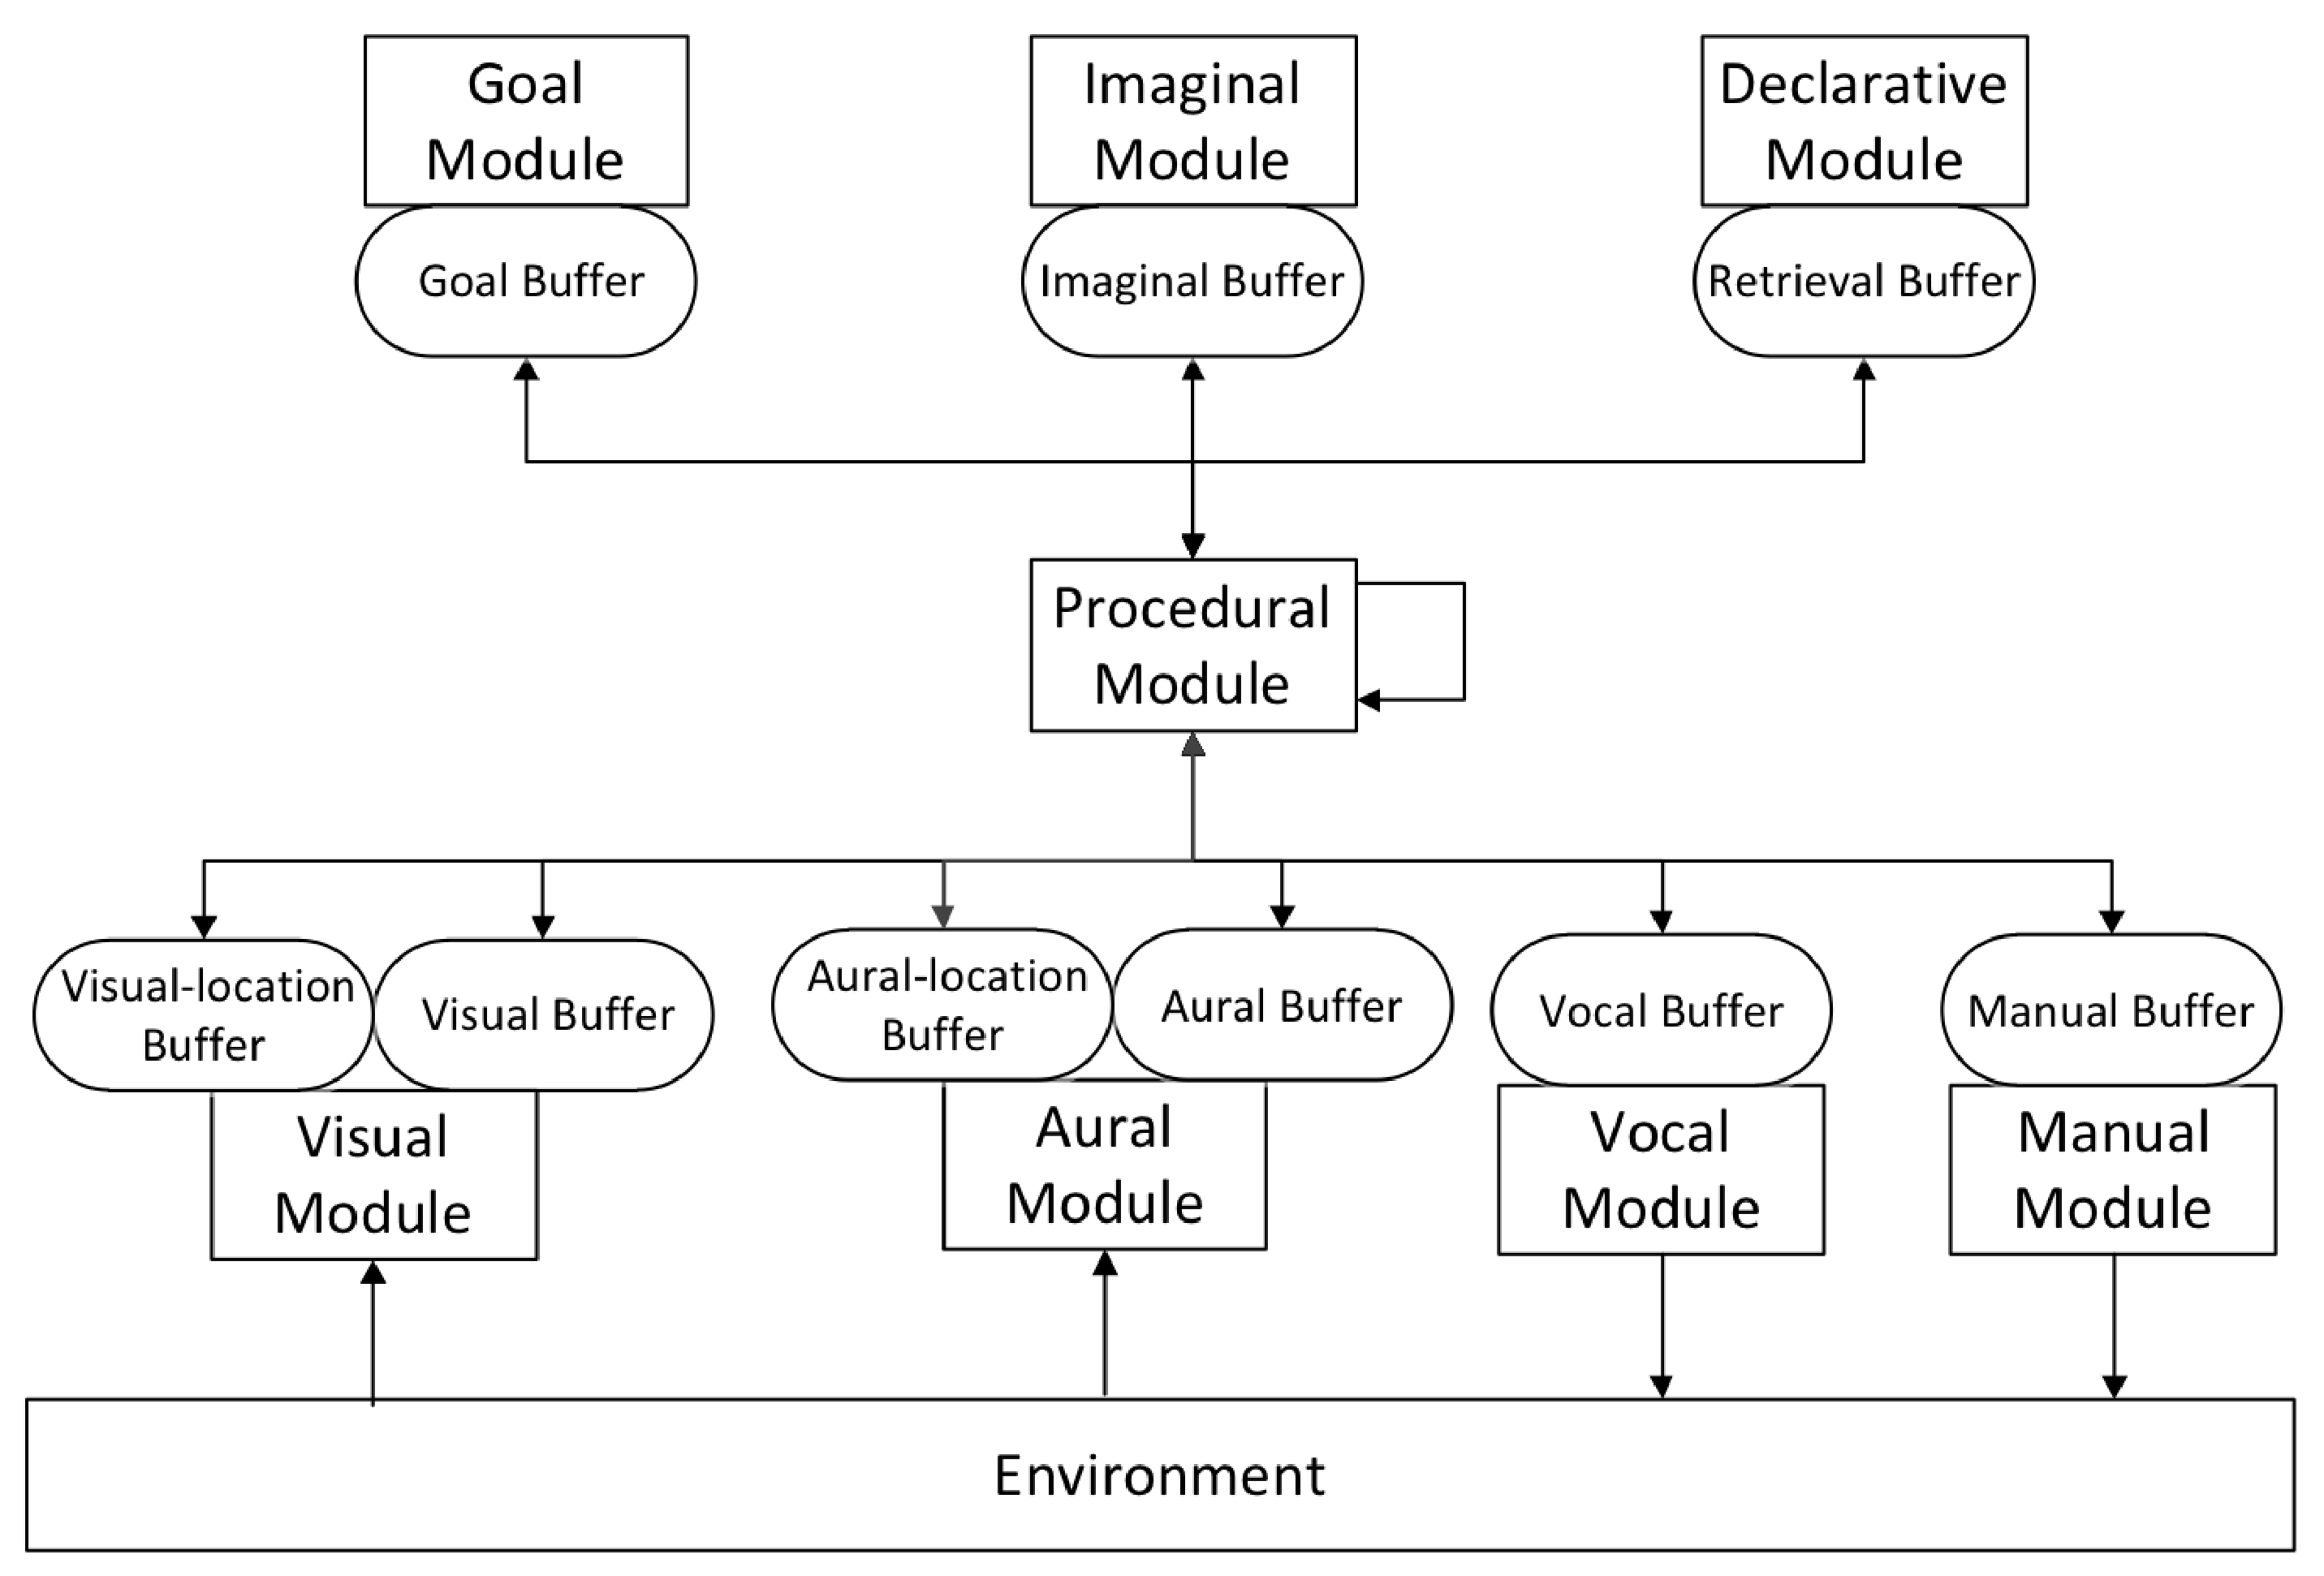
\includegraphics[scale=0.25]{images/ch_01/actr.eps}
	  \end{center} 
	  \caption{\textit{Structure of Act-r.}}  
	  \label{fig:modulesActr}
	\end{figure}
	
	Each module is independent from the others, to communicate one to each other they need to pass through the procedural module. As shown in Figure  ~\ref{fig:modulesActr} a module can have more than one buffer; for example, the aural module has two buffers: one is the "Aural-location Buffer", whose function is to get the focus about changes happened in the environment; the second is the "Aural Buffer", to get the real information about the environment.

	The buffers are the built in interface between modules, used to exchange chunks between them. Every buffer belongs to a module, while a module can also have no buffers. Each buffer can hold one chunk at a time, which is readable by the other modules, the guidelines say that a buffer can be written only by its owner. 

	Although the modules could work in parallel, their interaction is limited to a serial exchange of chunks. The modules usually work in a parallel way, but their interaction is only serial. There are two reasons for this limitation: firstly the structure of the buffers can hold only one chunk; secondly only one production which preconditions are satisfied can be fired. When the preconditions of more than one production are satisfied, the one to be fired is the one with the higher \emph{utility value}. This is a numeric quantity, it can be associated with each production in advance or it can be learned while the model runs.
	
	From an informatics point of view \mbox{ACT-R} is a software written in Lisp and its models are written in a Lisp-like language. It is thought to have a modular structure so that it can be easily extended. \mbox{ACT-R 6.0} is the implementation of a state of the ars theory of human cognition, developed by John R. Anderson. Anderson credits Allen Newell as source of influence to his theory.
	
	
  %% OPENCV
  \section{OpenCV}
	\mbox{OpenCV}, an abbreviation that stands for \emph{Open Source Computer Vision}, is a computer vision library that was originally developed by Intel and, later on, by Willow Garage.
	It is a cross-platform library, released under a BSD license, thus it is free and open source. In the beginning it was developed in C and C++ and afterwards it was expanded by the addition of interfaces for Java and Python. \mbox{OpenCV} is designed for computational efficiency and with a strong focus on real-time applications. The version 2.4 has more than 2500 algorithms. The library has been used in many applications as, for example, mine inspection and robotics \cite{OpenCV:MainWebPage}. The following sections contain a brief history of the library and a list of its main features.
		
	\subsubsection*{History}
	The \mbox{OpenCV} Project started in 1999 as an Intel Reasearch initiative aimed to improve CPU intensive applications as a part of projects including real-time ray tracing and 3D display walls. The early goals of the project were developing optimized code for basic vision infrastructure, spreading this infrastructure to developers and making it portable and available for free, using a license that let the developers create both commercial and free applications.\newline
	The first alpha version was released to the public in 2000, followed by five beta versions between 2001 and 2005, which lead to version 1.0 in 2006. In 2008, the technology incubator Willow Garage begun supporting the project and, in the same year, version 1.1  was released.
	In October 2009, \mbox{OpenCV} 2.0 was released. It includes many improvements, such as a better C++ interface, more programming patterns, new functions and an optimization for multi-core architectures. According to the current \mbox{OpenCV} release plan, a new version of the library is delivered on a six-months basis. \cite{OpenCV:ChangeLogs}.
	
	\subsubsection*{Main Features}
	\mbox{OpenCV} offers a wide range of possibilities. First of all, it provides an easy way to manage image and video data types. It also offers functions to load, copy, edit, convert and store images and a basic graphical user interface that lets the developers handle keyboard and mouse and display images and videos. The library lets manipulate images even with matrix and vector algebra routines. It supports the most common dynamic data structures and offers many different basic image processing functions: filtering, edge and corner detection, color conversion, sampling and interpolation, morphological operations, histograms and image pyramids. Beyond this, it integrates many functions for structural analysis of the image, camera calibration, motion analysis and object recognition. \cite{Agam2006}.
